%! TEX root = ../main.tex
% ============================================================
% IMMUTABLE — generated automatically, do not edit this block
%   script          : plotter.py::plot_td_vs_fft
%   plot_type       : td_vs_fft
%   chapter         : 04
%   panel           : None
%   wind            : None
%   amplitude       : None
%   frequency       : None
%   probes          : 9373/170, 12400/250, 9373/340, 8804/250
%   draft           : True
%
% DATASETS:
%   PROCESSED-20260326-ProbePos4_31_FPV_2-tett6roof-under9Mooring-height100-lowrange
%   PROCESSED-20260327-ProbePos4_31_FPV_2-tett6roof-under9Mooring30-height100-lowrange
%
% SUBFIGURES AVAILABLE:
%   FIGURES/ch04_td_vs_fft_scatter.pdf
% ============================================================
\begin{figure}[htbp]
  \centering
  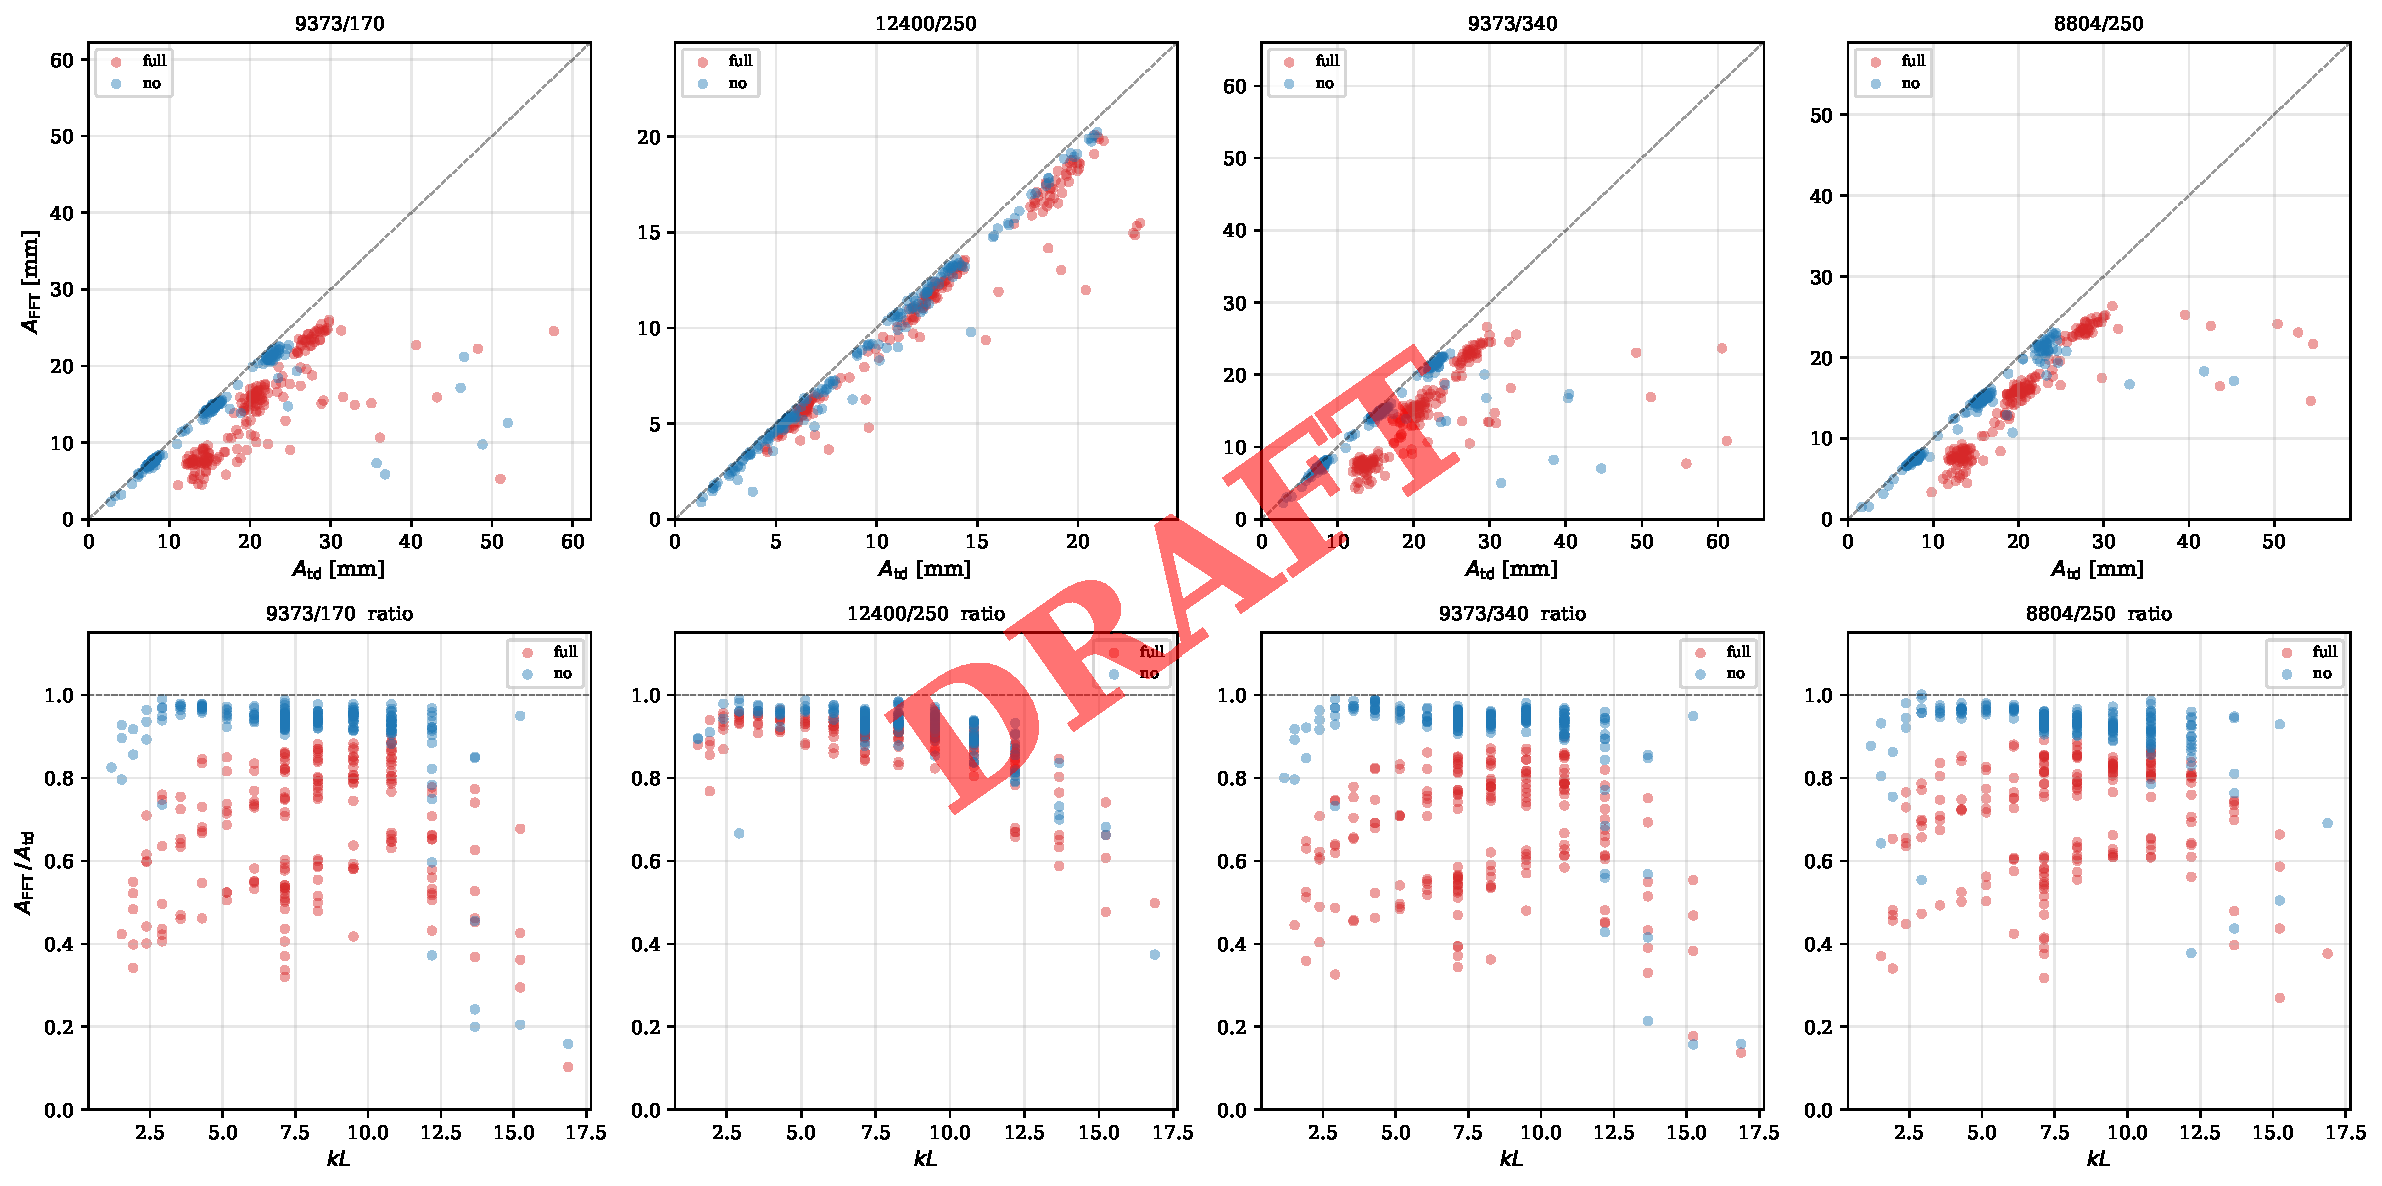
\includegraphics[width=0.9\linewidth]{FIGURES/ch04_td_vs_fft_scatter.pdf}
  \caption[Same data as the td-vs-fft figure]{
    Same data as the td-vs-fft figure. Bottom row: individual run ratios as scatter (no median line). Use to identify outlier runs driving dips at specific kL.
  }
  \label{fig:ch04_td_vs_fft_scatter}
\end{figure}
